\documentclass[letterpaper,12pt]{article}
\usepackage[bottom=2.5cm, top=2.5cm, right=2cm, left=3cm]{geometry}
\usepackage[spanish, es-tabla]{babel}
\usepackage{graphicx} 
\usepackage{hyperref}
\usepackage{booktabs}
\usepackage{natbib}
\usepackage{float}
\usepackage{listings}
\usepackage{xcolor}
\usepackage{parskip} 
\usepackage{fancyhdr} % Paquete para personalizar encabezados y pies de página
\usepackage{microtype}  % Mejora la justificación del texto

\hypersetup{
    colorlinks=true,
    linkcolor=black,
    citecolor=black,
    urlcolor=blue
}

% Configuración del encabezado
\pagestyle{fancy}
\fancyhf{} % Limpia los encabezados y pies de página actuales
\fancyhead[R]{\thepage} % Coloca el número de página en la parte superior derecha
\renewcommand{\headrulewidth}{0pt} % Elimina la línea horizontal en la parte superior de la página

\begin{document}

\begin{titlepage}
    \begin{center}
        
    
    \vspace*{1cm}


    \textbf{\Large EVALUACIÓN SOCIAL BASADA EN REALIDAD}
  
    \vspace{1cm}
    
    \textbf{Bernardo Caprile Canala-Echevarría, Felipe Alberto Vicencio Fossa y Lukas Wolff Casanova}\\
    Facultad de Ingeniería y Ciencias Aplicadas, Universidad de los Andes, Santiago de Chile\\
    e-mail: \href{mailto:bcaprile@miuandes.cl}{bcaprile@miuandes.cl}, \href{mailto:favicencio@miuandes.cl}{favicencio@miuandes.cl}, \href{mailto:lwolff@miuandes.cl}{lwolff@miuandes.cl}\\
    GitHub: \href{https://github.com/LukasWolff2002/TAREA_4_AUTITOS}{Repositorio}
    \vspace{2cm}
    
    \textbf{ABSTRACT}
    \end{center}
    \vspace{0.5cm}
    
    The project evaluates an infrastructure improvement in San Carlos de Apoquindo, focusing on General Blanche and Camino El Alba avenues, which will operate as one-way roads to optimize traffic flow. This proposal reduces traffic conflicts by allocating three lanes per road, resulting in significant reductions in operational costs, travel times ($CT_i$), and fuel consumption ($CC$). The results show substantial improvements in network efficiency, particularly in key arcs such as $d$, with a strategic redistribution of traffic flow. The initial investment of 1 billion pesos yields estimated net social benefits of 403 million pesos, supporting the project's economic feasibility. This analysis, conducted using social evaluation methodologies and simulated data, highlights the proposal's positive impact in terms of savings and optimization. However, to make a more informed decision, it would be crucial to incorporate factors such as environmental impact, demand elasticity, and long-term indirect effects, which could influence the outcomes.


    \vspace{1cm}
    
    \textit{Key words:} \textit{Infrastructure, Traffic optimization, Cost efficiency, Social evaluation, Net benefits.}
    
\end{titlepage}

\newpage
\section{Introducción}

En este informe se tiene como objetivo evaluar socialmente la mejora de una propuesta en una red vial ficticia, inspirada en el sector de San Carlos de Apoquindo. El grafo de la Figura \ref{fig:imagen1} representa dicha red, donde los diferentes arcos y centroides simbolizan avenidas y puntos clave de la zona. 


\begin{figure}[h]
    \centering
    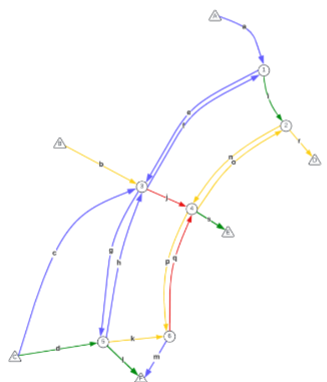
\includegraphics[width=0.3\textwidth]{FOTOS/diagrama.png}
    \caption{Diagrama de la red vial ficticia}
    \label{fig:imagen1}
\end{figure}



La mejora propuesta consiste en reorganizar las avenidas General Blanche y Camino El Alba para operar en sentidos exclusivos (oriente y poniente, respectivamente), permitiendo la delimitación de tres pistas en cada vía y reduciendo conflictos de tránsito. Este cambio implica una modificación en la función de costo del arco $d$, que pasa a formar parte del conjunto amarillo con un parámetro $S = 2000$.

El análisis considera las metodologías de evaluación social vistas en clase, con un enfoque en los beneficios derivados de la reducción de tiempos de viaje durante horas punta. En los apartados siguientes, se detallan los datos base, la metodología aplicada, los cálculos realizados y las conclusiones obtenidas.

\newpage
\section{Resultados}

Lo primero que se calculó a partir de la base de datos de la propuesta inicial y la propuesta mejorada fueron los costos del tiempo, combustible y otros costos de cada arco. Estos datos se presentan en las Tablas \ref{tab:datos_actualizados} y \ref{tab:datos}.


\begin{equation}
    CT_i = FE_i \sum_{j=1}^{NV} (VT_j \cdot \sum_{k \epsilon A_j} q_{qjk} \cdot TV_{ijk} \cdot TO_{ijk})
\end{equation}

\begin{equation}
    CC_i = FE_i \sum_{j=1}^{NV} (VC_j \cdot \sum_{k \epsilon A_j} q_{qjk} \cdot [L_k cm_j(v_{ij})+h_{ik} cd_j(v_{ij})+ d_{ik}cr_j)])
\end{equation}

\begin{equation}
    OC_i = FE_i \sum_{j}\sum_{i} q_{ijk} L_k \cdot (CL_{ijk} \cdot VL_j + CN_{ijk} \cdot VN_j + CR_{ijk} \cdot VV_j+ CM_{ijk} \cdot VH_j) /1000
\end{equation}


\subsection{Datos de la propuesta base}


\begin{table}[H]
    \centering
    \caption{Tabla de datos de flujo, costo aproximado y costos adicionales de la propuesta incial}
    \begin{tabular}{ccccccc}
        \toprule
        \textbf{Arco} & \textbf{Flujo [veh]} & \textbf{Costo aprox. [h]} & \textbf{CTi} & \textbf{CC} & \textbf{OC} \\
        \midrule
        a & 1600.00 & 0.625 & 2.017872e+09 & 2.559557e+08 & 1.523648e+08 \\
        b & 2250.00 & 0.150 & 6.810318e+08 & 1.176139e+08 & 2.142630e+08 \\
        c & 1255.00 & 0.280 & 7.090802e+08 & 1.025944e+08 & 1.195111e+08 \\
        d & 1845.00 & 0.255 & 9.493583e+08 & 1.403678e+08 & 1.756956e+08 \\
        e & 710.31  & 0.025 & 3.583287e+07 & 1.699836e+07 & 6.764139e+07 \\
        f & 610.03  & 0.025 & 3.077406e+07 & 1.459857e+07 & 5.809193e+07 \\
        g & 605.30  & 0.025 & 3.053545e+07 & 1.448537e+07 & 5.764150e+07 \\
        h & 0.02    & 0.025 & 1.008936e+03 & 4.786180e+02 & 1.904560e+03 \\
        i & 1499.72 & 0.025 & 7.565607e+07 & 3.588965e+07 & 1.428153e+08 \\
        j & 3000.00 & 0.025 & 1.513404e+08 & 7.179270e+07 & 2.856840e+08 \\
        k & 785.28  & 0.025 & 3.961486e+07 & 1.879246e+07 & 7.478063e+07 \\
        l & 1665.00 & 0.135 & 4.535672e+08 & 8.137159e+07 & 1.585546e+08 \\
        m & 1085.00 & 0.110 & 2.408330e+08 & 4.687573e+07 & 1.033224e+08 \\
        n & 89.69   & 0.025 & 4.524573e+06 & 2.146362e+06 & 8.540998e+06 \\
        o & 1089.97 & 0.025 & 5.498550e+07 & 2.608396e+07 & 1.037956e+08 \\
        p & 694.70  & 0.025 & 3.504539e+07 & 1.662480e+07 & 6.615488e+07 \\
        q & 394.98  & 0.025 & 1.992548e+07 & 9.452227e+06 & 3.761315e+07 \\
        r & 2500.00 & 0.275 & 1.387287e+09 & 2.015371e+08 & 2.380700e+08 \\
        s & 1700.00 & 0.158 & 5.420004e+08 & 9.194747e+07 & 1.618876e+08 \\
        \bottomrule
    \end{tabular}
    \\
    Fuente: elaboración propia.
    \label{tab:datos_actualizados}
\end{table}

\newpage
\subsection{Datos de la propuesta mejorada}
\begin{table}[H]
    \centering
    \caption{Tabla de datos de flujo, costo aproximado y costos adicionales de la propuesta mejorada}
    \begin{tabular}{ccccccc}
        \toprule
        \textbf{Arco} & \textbf{Flujo [veh]} & \textbf{Costo aprox. [h]} & \textbf{CTi} & \textbf{CC} & \textbf{OC} \\
        \midrule
        a & 1600.00 & 0.625 & 2.017872e+09 & 2.559557e+08 & 1.523648e+08 \\
        b & 2250.00 & 0.150 & 6.810318e+08 & 1.176139e+08 & 2.142630e+08 \\
        c & 1050.00 & 0.075 & 1.589074e+08 & 3.703107e+07 & 9.998938e+07 \\
        d & 2050.00 & 0.050 & 2.068319e+08 & 6.067855e+07 & 1.952174e+08 \\
        e & 710.31  & 0.025 & 3.583287e+07 & 1.699836e+07 & 6.764139e+07 \\
        f & 610.03  & 0.025 & 3.077406e+07 & 1.459857e+07 & 5.809193e+07 \\
        g & 605.30  & 0.025 & 3.053545e+07 & 1.448537e+07 & 5.764150e+07 \\
        h & 102.52  & 0.025 & 5.171806e+06 & 2.453396e+06 & 9.762773e+06 \\
        i & 1499.72 & 0.025 & 7.565607e+07 & 3.588965e+07 & 1.428153e+08 \\
        j & 2897.50 & 0.025 & 1.461696e+08 & 6.933978e+07 & 2.759231e+08 \\
        k & 887.78  & 0.025 & 4.478566e+07 & 2.124537e+07 & 8.454150e+07 \\
        l & 1665.00 & 0.135 & 4.535672e+08 & 8.137159e+07 & 1.585546e+08 \\
        m & 1085.00 & 0.110 & 2.408330e+08 & 4.687573e+07 & 1.033224e+08 \\
        n & 89.69   & 0.025 & 4.524573e+06 & 2.146362e+06 & 8.540998e+06 \\
        o & 1089.97 & 0.025 & 5.498550e+07 & 2.608396e+07 & 1.037956e+08 \\
        p & 694.70  & 0.025 & 3.504539e+07 & 1.662480e+07 & 6.615488e+07 \\
        q & 497.48  & 0.025 & 2.509627e+07 & 1.190514e+07 & 4.737402e+07 \\
        r & 2500.00 & 0.275 & 1.387287e+09 & 2.015371e+08 & 2.380700e+08 \\
        s & 1700.00 & 0.158 & 5.420004e+08 & 9.194747e+07 & 1.618876e+08 \\
        \bottomrule
    \end{tabular}
    \\
    Fuente: elaboración propia.
    \label{tab:datos}
\end{table}

\begin{table}[H]
    \centering
    \caption{Variación de los costos por arco.}
    \begin{tabular}{ccccc}
        \toprule
        \textbf{Arco} & \textbf{Variación CTi} & \textbf{Variación CC} & \textbf{Variación OC} \\
        \midrule
        a & 0.0         & 0.000000e+00 & 0.000000e+00 \\
        b & 0.0         & 0.000000e+00 & 0.000000e+00 \\
        c & 550172800.8 & 6.556331e+07 & 1.952174e+07 \\
        d & 742526449.2 & 7.968926e+07 & -1.952174e+07 \\
        e & 0.0         & 0.000000e+00 & 0.000000e+00 \\
        f & 0.0         & 0.000000e+00 & 0.000000e+00 \\
        g & 0.0         & 0.000000e+00 & 0.000000e+00 \\
        h & -5170797.0  & -2.452917e+06 & -9.760868e+06 \\
        i & 0.0         & 0.000000e+00 & 0.000000e+00 \\
        j & 5170797.0   & 2.452917e+06 & 9.760868e+06 \\
        k & -5170797.0  & -2.452917e+06 & -9.760868e+06 \\
        l & 0.0         & 0.000000e+00 & 0.000000e+00 \\
        m & 0.0         & 0.000000e+00 & 0.000000e+00 \\
        n & 0.0         & 0.000000e+00 & 0.000000e+00 \\
        o & 0.0         & 0.000000e+00 & 0.000000e+00 \\
        p & 0.0         & 0.000000e+00 & 0.000000e+00 \\
        q & -5170797.0  & -2.452917e+06 & -9.760868e+06 \\
        r & 0.0         & 0.000000e+00 & 0.000000e+00 \\
        s & 0.0         & 0.000000e+00 & 0.000000e+00 \\
        \bottomrule
    \end{tabular}
    \\
    Fuente: elaboración propia.
    \label{tab:variacion_costos}
\end{table}


\begin{table}[H]
    \centering
    \caption{Resumen tabular de costos y ganancias del proyecto.}
    \begin{tabular}{ccc}
        \toprule
        \textbf{Costo del Proyecto} & \textbf{Variación Total de Costos} & \textbf{Ganancia Obtenida} \\
        \midrule
        1,000,000,000 & 1,403,182,654.38 & 403,182,654.38 \\
        \bottomrule
    \end{tabular}
    \\
    Fuente: elaboración propia.
    \label{tab:resumen_costos}
\end{table}

\newpage

\section{Discusiones}

El modelo presentado para evaluar la mejora vial tiene puntos fuertes, pero también simplificaciones que podrían afectar su precisión y aplicabilidad. Por un lado, se basa en una metodología clara para medir beneficios económicos, como la reducción de tiempos de viaje y costos operativos. Sin embargo, los supuestos adoptados simplifican la realidad de manera significativa.

Primero, considerar que todas las avenidas tienen una longitud de 1 km y una velocidad uniforme de 40 km/h ignora factores como pendientes, condiciones del pavimento o variaciones reales en el tráfico. Esto podría llevar a estimaciones inexactas de costos y beneficios.

Segundo, aunque el modelo utiliza el equilibrio de Wardrop para la redistribución del flujo vehicular, no evalúa cómo cambios a largo plazo, como el aumento de la demanda inducida, podrían afectar los resultados. Tampoco se analiza el impacto en áreas cercanas ni posibles desventajas como nuevos puntos de congestión.

Además, al enfocarse únicamente en horas punta, se dejan fuera beneficios o costos que ocurren durante el resto del día, como la reducción de emisiones o el desgaste de la infraestructura. También falta considerar impactos sociales como la seguridad vial o efectos sobre peatones y ciclistas.

Los resultados sugieren que la mejora es económicamente viable, con beneficios netos importantes. Sin embargo, para tomar una decisión más informada sería necesario un análisis más completo, incluyendo impactos ambientales, patrones de tráfico a largo plazo y cómo esta inversión se alinea con otros objetivos de transporte sostenible.

Finalizando, aunque el modelo es un buen inicio, necesita mayor detalle para asegurar que los beneficios superen los costos a nivel económico, social y ambiental.

\newpage

\section{Conclusiones}

En conclusión, la propuesta de mejora vial muestra buenos resultados económicos, con beneficios claros y una mejor organización del tráfico en la red. Sin embargo, para estar seguros de que la inversión será realmente positiva a largo plazo, es importante incluir un análisis más completo. Esto debería considerar el impacto ambiental, los efectos sociales y cómo podría cambiar la demanda en el futuro. Con estos aspectos, se podría tomar una decisión más completa y alineada con objetivos como la sostenibilidad y el bienestar de la comunidad. Así, se aseguraría que los beneficios del proyecto sean duraderos y para todos.


\end{document}